% \documentclass[table]{beamer}
\documentclass[table,handout]{beamer}
\setbeameroption{show notes}
% \setbeameroption{hide notes}
% \setbeameroption{show only notes}
\usepackage{varwidth}

\newif\ifhide
\newif\ifpost
\newif\ifhideclicker

% \hidetrue
% \hideclickertrue
% \posttrue

\newcommand{\whiteout}[1]{\textcolor{white}{#1}}
% \newcommand{\whiteoutbox}[1]{\fcolorbox{white}{white}{\parbox{\dimexpr \linewidth-2\fboxsep-2\fboxrule}{\whiteout{#1}}}}
% \newcommand{\notebox}[1]{\fcolorbox{blue}{white}{\parbox{\dimexpr \linewidth-2\fboxsep-2\fboxrule}{#1}}}
\newcommand{\whiteoutbox}[1]{\fcolorbox{white}{white}{\parbox{\linewidth}{\whiteout{#1}}}}
\newcommand{\notebox}[1]{\fcolorbox{blue}{white}{\parbox{\linewidth}{#1}}}
\newcommand{\blankbox}[1]{\phantom{\varwidth{\linewidth}\whiteoutbox{#1}\endvarwidth}}
\newcommand{\blank}[1]{\phantom{\varwidth{\linewidth}#1\endvarwidth}}

\ifhide%
    \newcommand{\hmask}[1]{\blank{#1}}%
\else%
    \newcommand{\hmask}[1]{#1}%
\fi

\ifhide%
    \newcommand{\wout}[1]{\whiteout{#1}}%
\else%
    \newcommand{\wout}[1]{#1}%
\fi

\ifhide%
    \newcommand{\hignore}[1]{}%
\else%
    \newcommand{\hignore}[1]{#1}%
\fi

\ifpost%
    \newcommand{\nopost}[1]{}%
\else%
    \newcommand{\nopost}[1]{#1}%
\fi

\ifhideclicker%
    \newcommand{\clickerslide}[1]{\stepcounter{clickerQuestionCounter}%
        \begin{frame}[t]
            \textcolor{blue}{Q \arabic{clickerQuestionCounter}:}
        \end{frame}}
\else%
    \newcommand{\clickerslide}[1]{#1}%
\fi

\ifhide%
    \newcommand{\hidebox}[1]{\blank{#1}}%
\else%
    \newcommand{\hidebox}[1]{\notebox{#1}}%
\fi

\ifhide%
    \newcommand{\wbox}[1]{\whiteoutbox{#1}}%
\else%
    \newcommand{\wbox}[1]{\notebox{#1}}%
\fi

\ifhide%
    \newcommand{\nbox}[1]{\blankbox{#1}}%
\else%
    \newcommand{\nbox}[1]{\notebox{#1}}%
\fi

\ifhideclicker%
    \newcommand{\clickeranswer}[1]{#1}%
\else%
    \ifhide%
        \newcommand{\clickeranswer}[1]{#1}%
    \else%
        \newcommand{\clickeranswer}[1]{\textbf{\textcolor{blue}{#1}}}%
    \fi
\fi

\usepackage{beamerthemesplit}
% \usetheme{boxes}
\usetheme{Malmoe}
\usecolortheme{seahorse}
% \usecolortheme{seagull}
\usepackage{ifthen}
\usepackage{xspace}
\usepackage{multirow}
\usepackage{multicol}
\usepackage{booktabs}
\usepackage{xcolor}
\usepackage{wasysym}
\usepackage{comment}
\usepackage{hyperref}
\hypersetup{pdfborder={0 0 0}, colorlinks=true, urlcolor=blue, linkcolor=blue, citecolor=blue}
\usepackage{changepage}
\usepackage[compatibility=false]{caption}
\captionsetup[figure]{font=scriptsize, labelformat=empty, textformat=simple, justification=centering, skip=2pt}
\usepackage{tikz}
\usetikzlibrary{trees,calc,backgrounds}

\usepackage[bibstyle=joaks-slides,maxcitenames=3,mincitenames=1,backend=biber]{biblatex}

\newrobustcmd*{\shortfullcite}{\AtNextCite{\renewbibmacro{title}{}\renewbibmacro{in:}{}\renewbibmacro{number}{}}\fullcite}

\newrobustcmd*{\footlessfullcite}{\AtNextCite{\renewbibmacro{title}{}\renewbibmacro{in:}{}}\footfullcite}

% Make all footnotes smaller
% \renewcommand{\footnotesize}{\scriptsize}

\definecolor{myGray}{gray}{0.9}
\colorlet{rowred}{red!30!white}

\setbeamertemplate{blocks}[rounded][shadow=true]

\setbeamercolor{defaultcolor}{bg=structure!30!normal text.bg,fg=black}
\setbeamercolor{block body}{bg=structure!30!normal text.bg,fg=black}
\setbeamercolor{block title}{bg=structure!50!normal text.bg,fg=black}

\newenvironment<>{varblock}[2][\textwidth]{%
  \setlength{\textwidth}{#1}
  \begin{actionenv}#3%
    \def\insertblocktitle{#2}%
    \par%
    \usebeamertemplate{block begin}}
  {\par%
    \usebeamertemplate{block end}%
  \end{actionenv}}

\newenvironment{displaybox}[1][\textwidth]
{
    \centerline\bgroup\hfill
    \begin{beamerboxesrounded}[lower=defaultcolor,shadow=true,width=#1]{}
}
{
    \end{beamerboxesrounded}\hfill\egroup
}

\newenvironment{onlinebox}[1][4cm]
{
    \newbox\mybox
    \newdimen\myboxht
    \setbox\mybox\hbox\bgroup%
        \begin{beamerboxesrounded}[lower=defaultcolor,shadow=true,width=#1]{}
    \centering
}
{
    \end{beamerboxesrounded}\egroup
    \myboxht\ht\mybox
    \raisebox{-0.25\myboxht}{\usebox\mybox}\hspace{2pt}
}

\newenvironment{mydescription}{
    \begin{description}
        \setlength{\leftskip}{-1.5cm}}
    {\end{description}}

\newenvironment{myitemize}{
    \begin{itemize}
        \setlength{\leftskip}{-.3cm}}
    {\end{itemize}}

% footnote without a marker
\newcommand\barefootnote[1]{%
  \begingroup
  \renewcommand\thefootnote{}\footnote{#1}%
  \addtocounter{footnote}{-1}%
  \endgroup
}

% define formatting for footer
\newcommand{\myfootline}{%
    {\it
    \insertshorttitle
    \hspace*{\fill} 
    \insertshortauthor, \insertshortinstitute
    % \ifx\insertsubtitle\@empty\else, \insertshortsubtitle\fi
    \hspace*{\fill}
    \insertframenumber/\inserttotalframenumber}}

% set up footer
\setbeamertemplate{footline}{%
    \usebeamerfont{structure}
    \begin{beamercolorbox}[wd=\paperwidth,ht=2.25ex,dp=1ex]{frametitle}%
        % \Tiny\hspace*{4mm}\myfootline\hspace{4mm}
        \tiny\hspace*{4mm}\myfootline\hspace{4mm}
    \end{beamercolorbox}}

% remove navigation bar
\beamertemplatenavigationsymbolsempty

\makeatletter
    \newenvironment{noheadline}{
        \setbeamertemplate{headline}[default]
        \def\beamer@entrycode{\vspace*{-\headheight}}
    }{}
\makeatother

\newcounter{clickerQuestionCounter}
\ifhideclicker%
\newenvironment{clickerquestion}
{ \stepcounter{clickerQuestionCounter}
  \begin{enumerate}[Q \arabic{clickerQuestionCounter}:]\color{white} }
{ \end{enumerate} }
\else%
\newenvironment{clickerquestion}
{ \stepcounter{clickerQuestionCounter}
  \begin{enumerate}[Q \arabic{clickerQuestionCounter}:] }
{ \end{enumerate} }
\fi

\ifhideclicker%
\newenvironment{clickeroptions}
{ \begin{enumerate}[\begingroup\color{white} 1)\endgroup]\color{white} }
{ \end{enumerate} }
\else%
\newenvironment{clickeroptions}
{ \begin{enumerate}[\begingroup\color{red} 1)\endgroup] }
{ \end{enumerate} }
\fi


\tikzstyle{centered} = [align=center, text centered, font=\sffamily\bfseries]
\tikzstyle{skip} = [centered, inner sep=0pt, fill]
\tikzstyle{empty} = [centered, inner sep=0pt]
\tikzstyle{inode} = [centered, circle, minimum width=4pt, fill=black, inner sep=0pt]
\tikzstyle{tnode} = [centered, circle, inner sep=1pt]
\tikzset{
  % edge styles
  level distance=10mm,
  mate/.style={edge from parent/.style={draw,distance=3pt}},
  mleft/.style={grow=left, level distance=10mm, edge from parent path={(\tikzparentnode.west)--(\tikzchildnode.east)}},
  mright/.style={grow=right, level distance=10mm, edge from parent path={(\tikzparentnode.east)--(\tikzchildnode.west)}},
  % node styles
  male/.style={rectangle,minimum size=4mm,fill=gray!80},
  female/.style={circle,minimum size=4mm,fill=gray!80},
  amale/.style={male,fill=red},
  afemale/.style={female,fill=red},
}

\newcommand{\highlight}[1]{\textcolor{violet}{\textit{\textbf{#1}}}}
\newcommand{\super}[1]{\ensuremath{^{\textrm{\sffamily #1}}}}
\newcommand{\sub}[1]{\ensuremath{_{\textrm{\sffamily #1}}}}
\newcommand{\dC}{\ensuremath{^\circ{\textrm{C}}}}
\newcommand{\tb}{\hspace{2em}}
\providecommand{\e}[1]{\ensuremath{\times 10^{#1}}}
\newcommand{\myHangIndent}{\hangindent=5mm}

\newcommand{\spp}[1]{\textit{#1}}

\newcommand\mybullet{\leavevmode%
\usebeamertemplate{itemize item}\hspace{.5em}}

\makeatletter
\newcommand*{\rom}[1]{\expandafter\@slowromancap\romannumeral #1@}
\makeatother

\newcommand{\blankslide}{{\setbeamercolor{background canvas}{bg=black}
\setbeamercolor{whitetext}{fg=white}
\begin{frame}<handout:0>[plain]
\end{frame}}}

\newcommand{\whiteslide}{
\begin{frame}<handout:0>[plain]
\end{frame}}

\newcommand{\f}[1]{\ensuremath{F_{#1}}}
\newcommand{\x}[1]{X\ensuremath{^{#1}}}
\newcommand{\y}[1]{Y\ensuremath{^{#1}}}

% Population growth macros
\newcommand{\popsize}[1]{\ensuremath{N_{#1}}}
\newcommand{\popgrowthratediscrete}[1]{\ensuremath{\lambda_{#1}}}
\newcommand{\popgrowthrate}[1]{\ensuremath{r_{#1}}}
\newcommand{\ptime}{\ensuremath{t}\xspace}

\tikzset{hide on/.code={\only<#1>{\color{white}}}}
\tikzset{
    invisible/.style={opacity=0},
    visible on/.style={alt={#1{}{invisible}}},
    alt/.code args={<#1>#2#3}{%
        \alt<#1>{\pgfkeysalso{#2}}{\pgfkeysalso{#3}}
        % \pgfkeysalso doesn't change the path
    },
}

% \bibliography{../bib/references}
\bibliography{references}
\author[J.\ Oaks]{
    %Jamie R.\ Oaks\inst{1}
    Jamie R.\ Oaks
}
\institute[BIOL 180]{
    \inst{}%
        BIOL 180: Introductory Biology
}



\title[Inferring Phylogenies]{Inferring Phylogenies}
% \date{\today}
\date{April 29, 2015}

\begin{document}

% \maketitle
\begin{noheadline}
\begin{frame}
    \begin{columns}[c]
        \column{.5\textwidth}
            \maketitle
        \column{.5\textwidth}
            \begin{figure}
                \begin{center}
                \includegraphics[width=\textwidth]{../images/darwin-tol-copyright-boris-kulikov-2007.jpg}
                \caption{\tiny \copyright~2007 Boris Kulikov \href{http://boris-kulikov.blogspot.com/}{boris-kulikov.blogspot.com}}
                \end{center}
            \end{figure}
    \end{columns}
\end{frame}
\end{noheadline}

\nopost{
\begin{noheadline}
\begin{frame}[c]
    \vspace{-6mm}
    \begin{center} 
        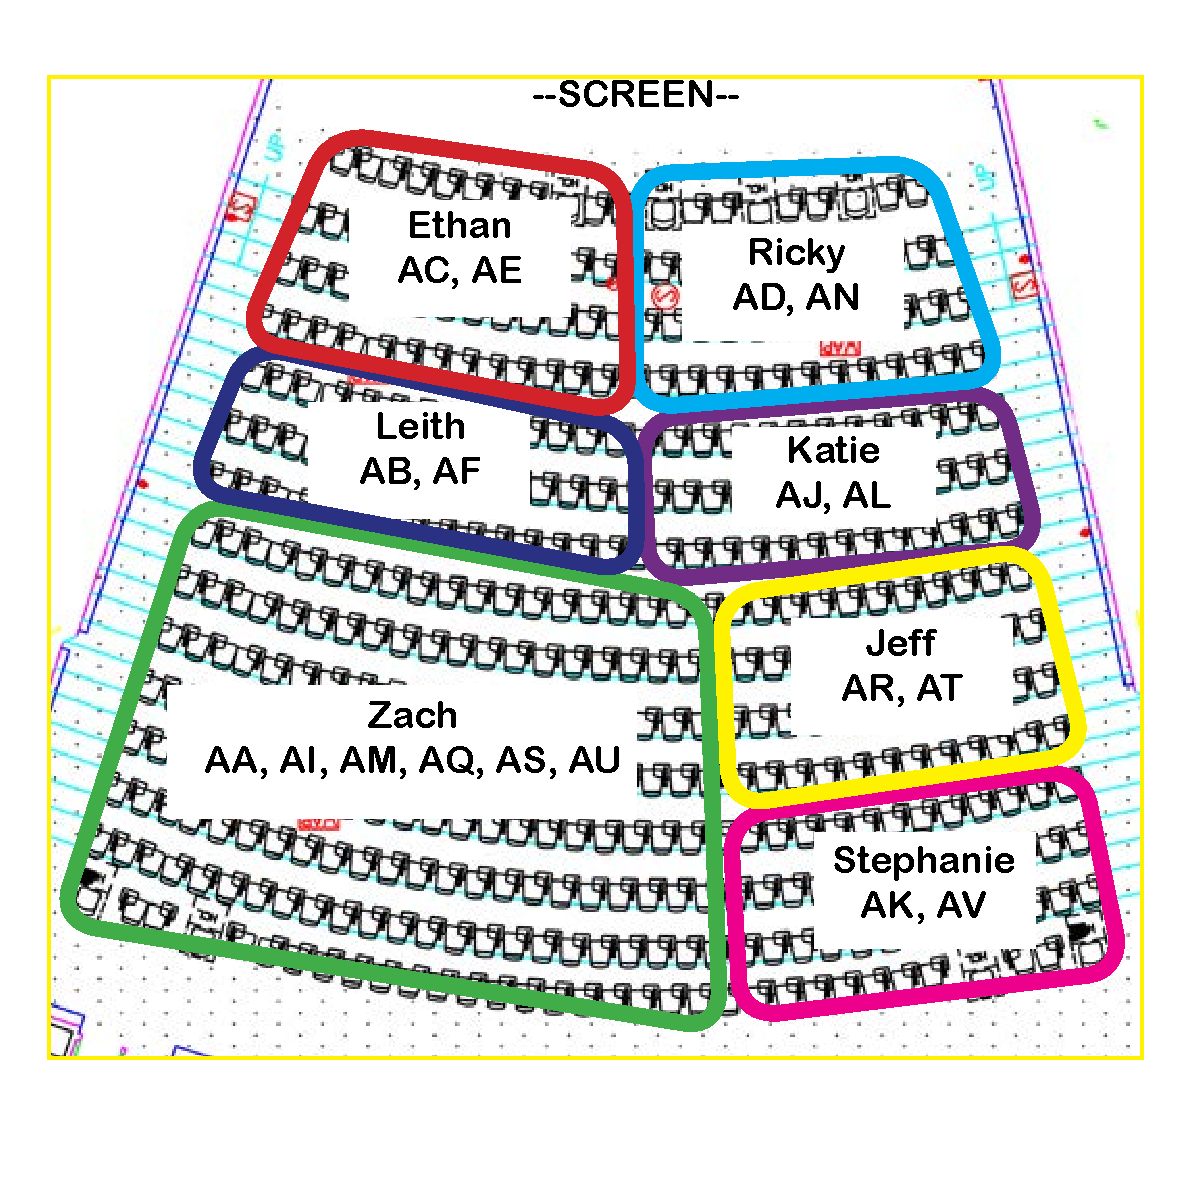
\includegraphics[height=1.2\textheight]{../images/seating-chart.pdf}
    \end{center}
\end{frame}
\end{noheadline}
}

\begin{noheadline}
\begin{frame}
    \begin{columns}[c]
        \column{.5\textwidth}
            Today's issues:
            \tableofcontents[subsectionstyle=hide]
        \column{.5\textwidth}
            \begin{figure}
                \begin{center}
                \includegraphics[width=\textwidth]{../images/darwin-tol-copyright-boris-kulikov-2007.jpg}
                \caption{\tiny \copyright~2007 Boris Kulikov \href{http://boris-kulikov.blogspot.com/}{boris-kulikov.blogspot.com}}
                \end{center}
            \end{figure}
    \end{columns}
\end{frame}
\end{noheadline}


%%%%%%%%%%%%%%%%%%%%%%%%%%%%%%%%%%%%%%%%%
\section{Why is phylogenetics important?}
%%%%%%%%%%%%%%%%%%%%%%%%%%%%%%%%%%%%%%%%%

% \begin{frame}
%     % \frametitle{Why is phylogenetics important?}
%     \begin{quote}
%     Seen in the light of evolution, biology is, perhaps, intellectually the
%     most satisfying and inspiring science. Without that light it becomes a pile
%     of sundry facts some of them interesting or curious but making no
%     meaningful picture as a whole.
%     \end{quote}

%     \myHangIndent
%     - Dobzhansky, T. (1973). Nothing in biology makes sense except in the light
%     of evolution. The American Biology Teacher 35:125--129.

%     \bigskip

%     \begin{quote}
%     \ldots nothing in evolution makes sense except in the light of phylogeny \ldots
%     \end{quote}

%     \myHangIndent
%     - Society of Systematic Biologists
% \end{frame}

\begin{frame}[t]
    % \frametitle{Why is phylogenetics important?}
    \begin{adjustwidth}{-1.5em}{-1.5em}
    We cannot understand biodiversity without its blueprint: the tree of life.
    \begin{columns}

        \column{0.5\linewidth}

        \begin{itemize}[<+->]
            \item Every field of biology studies organisms.
            \item These organisms are \textbf{not} independent.
            \item To analyze biological data correctly we need to account for
                shared history among organisms.
        \end{itemize}

        \column{0.5\linewidth}
        \begin{figure}
            \begin{center}
            % 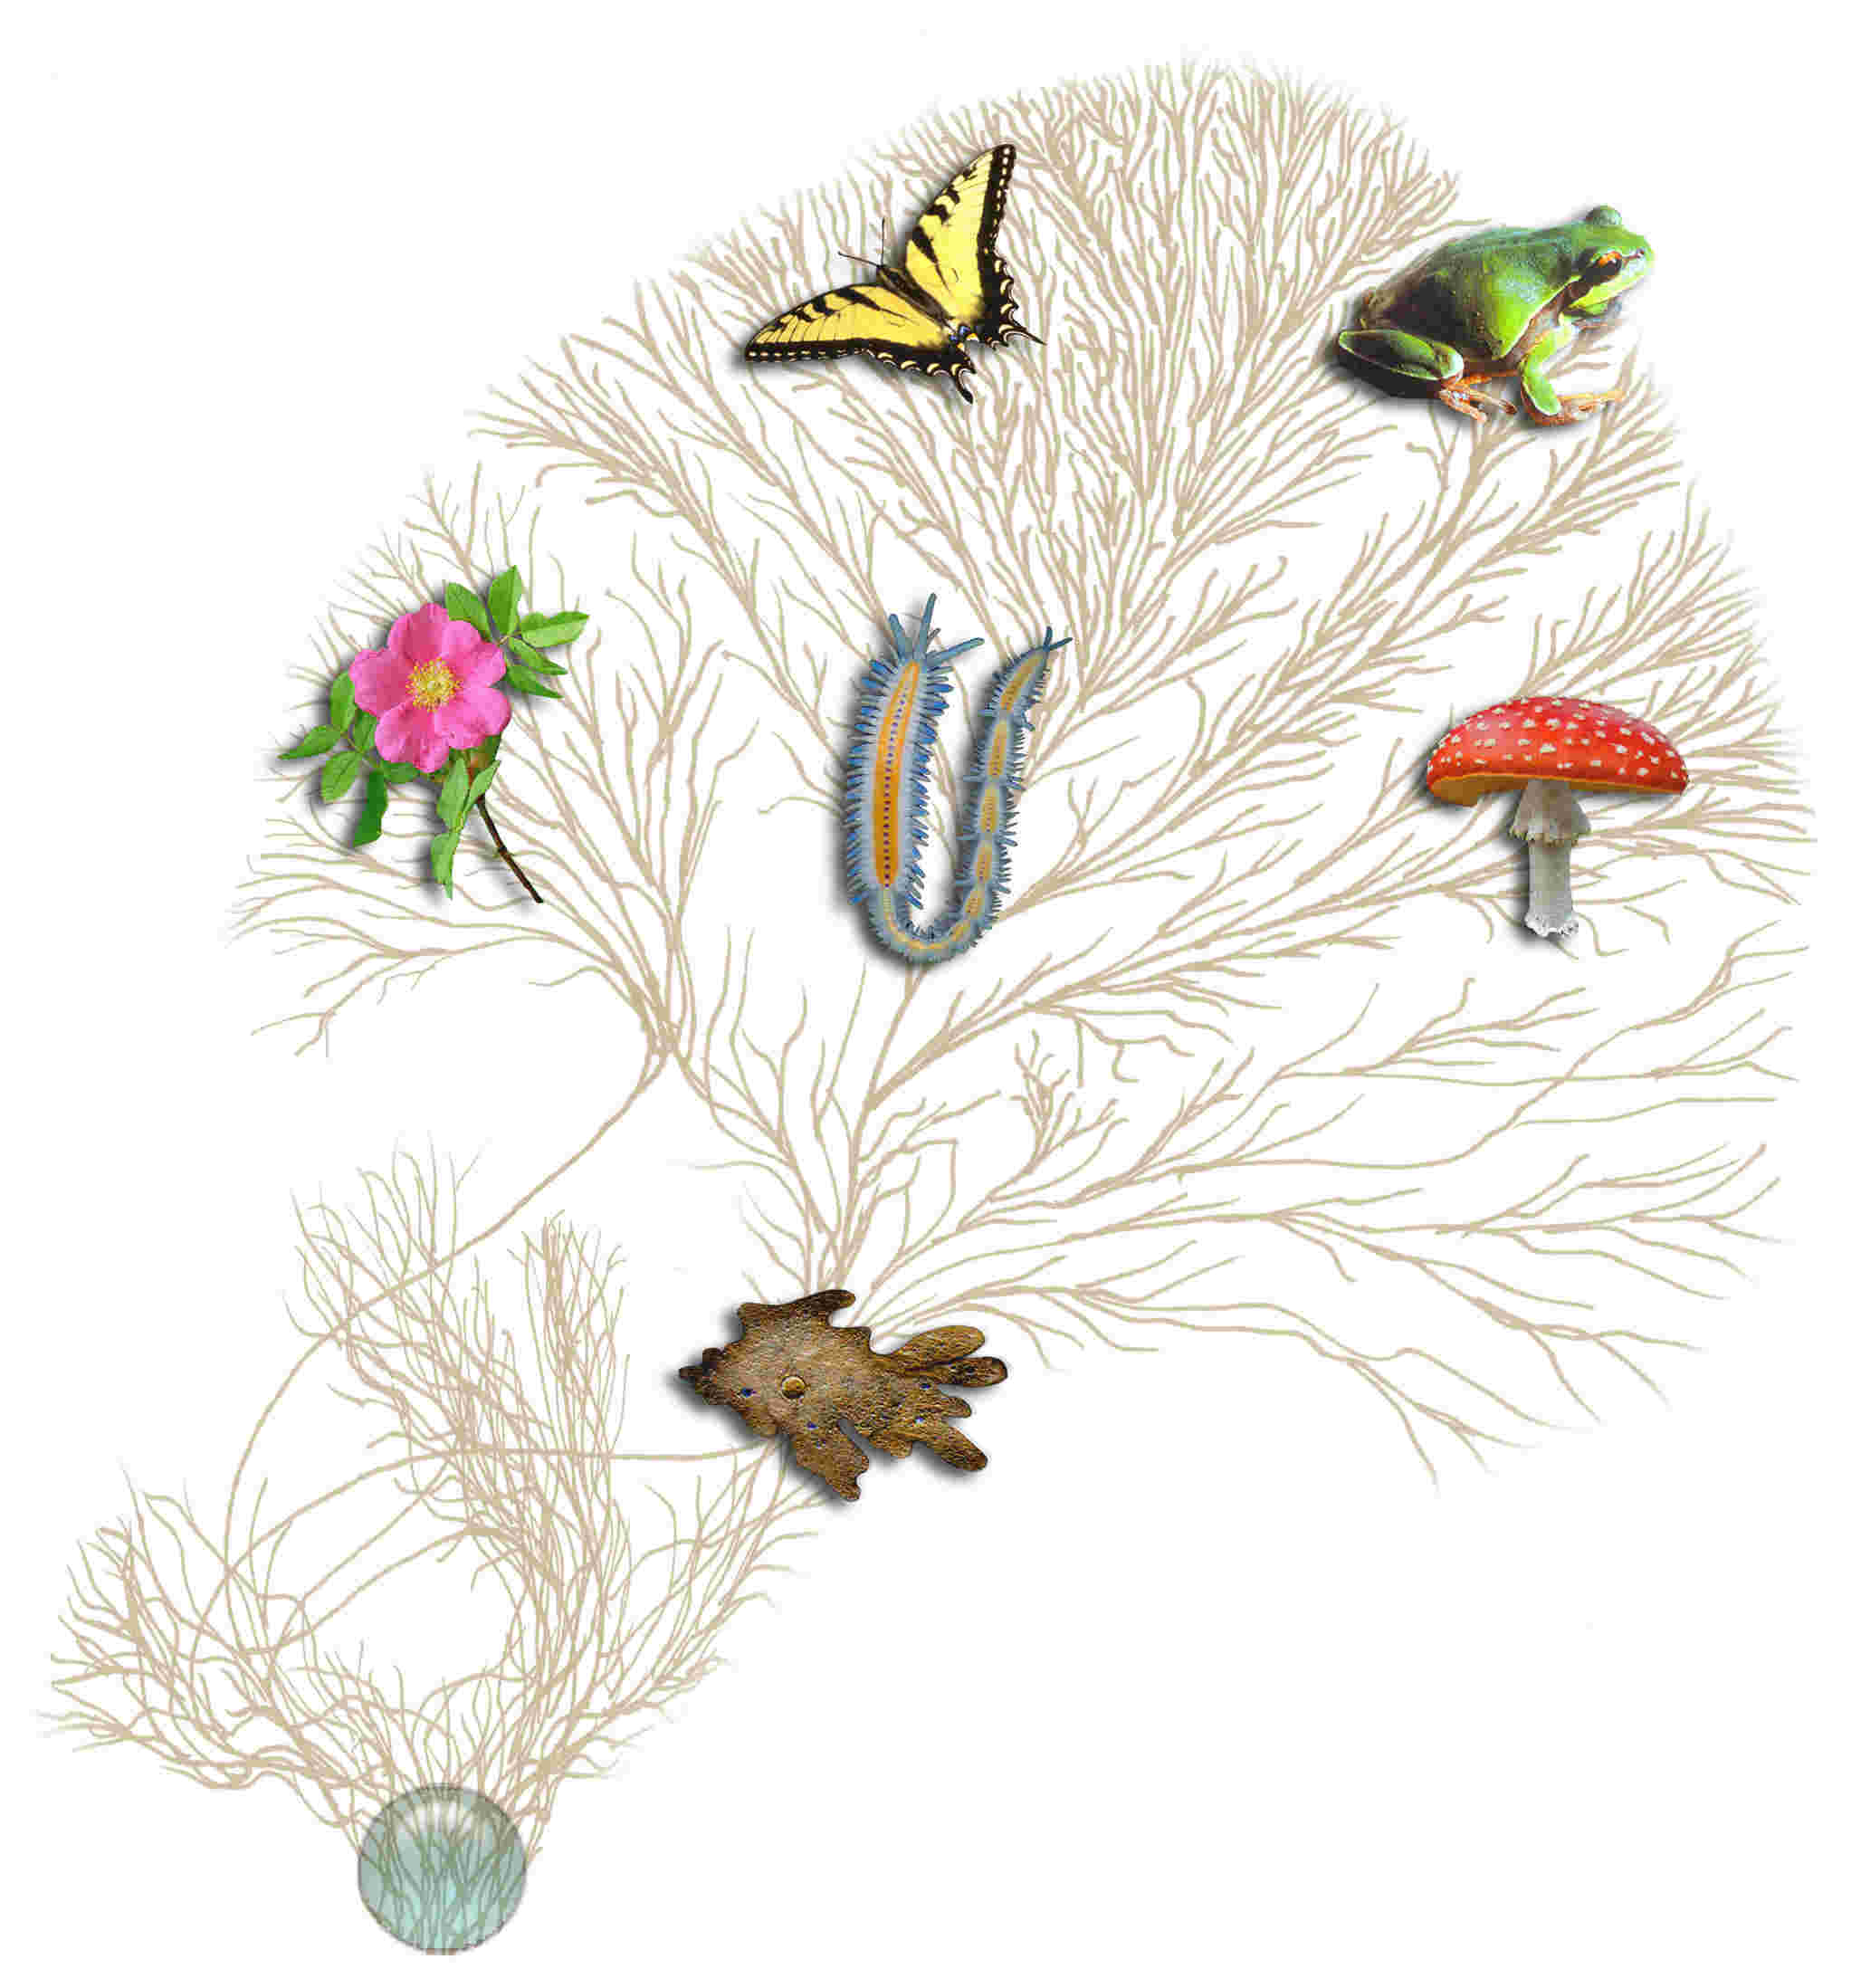
\includegraphics[width=0.95\textwidth]{../images/treeoflife.jpg}
            % \caption{\tiny \copyright~2007 Tree of Life Web Project \href{http://tolweb.org/tree/}{tolweb.org}}
            \includegraphics[width=0.95\textwidth]{../images/hillis-tree.pdf}
            \caption{\tiny \href{http://www.zo.utexas.edu/faculty/antisense/downloadfilestol.html}{Hillis Lab}}
            \end{center}
        \end{figure}
    
    \end{columns}
    \end{adjustwidth}
\end{frame}

% \begin{frame}
%     \frametitle{West Nile Virus}
%     \begin{figure}
%         \begin{center}
%         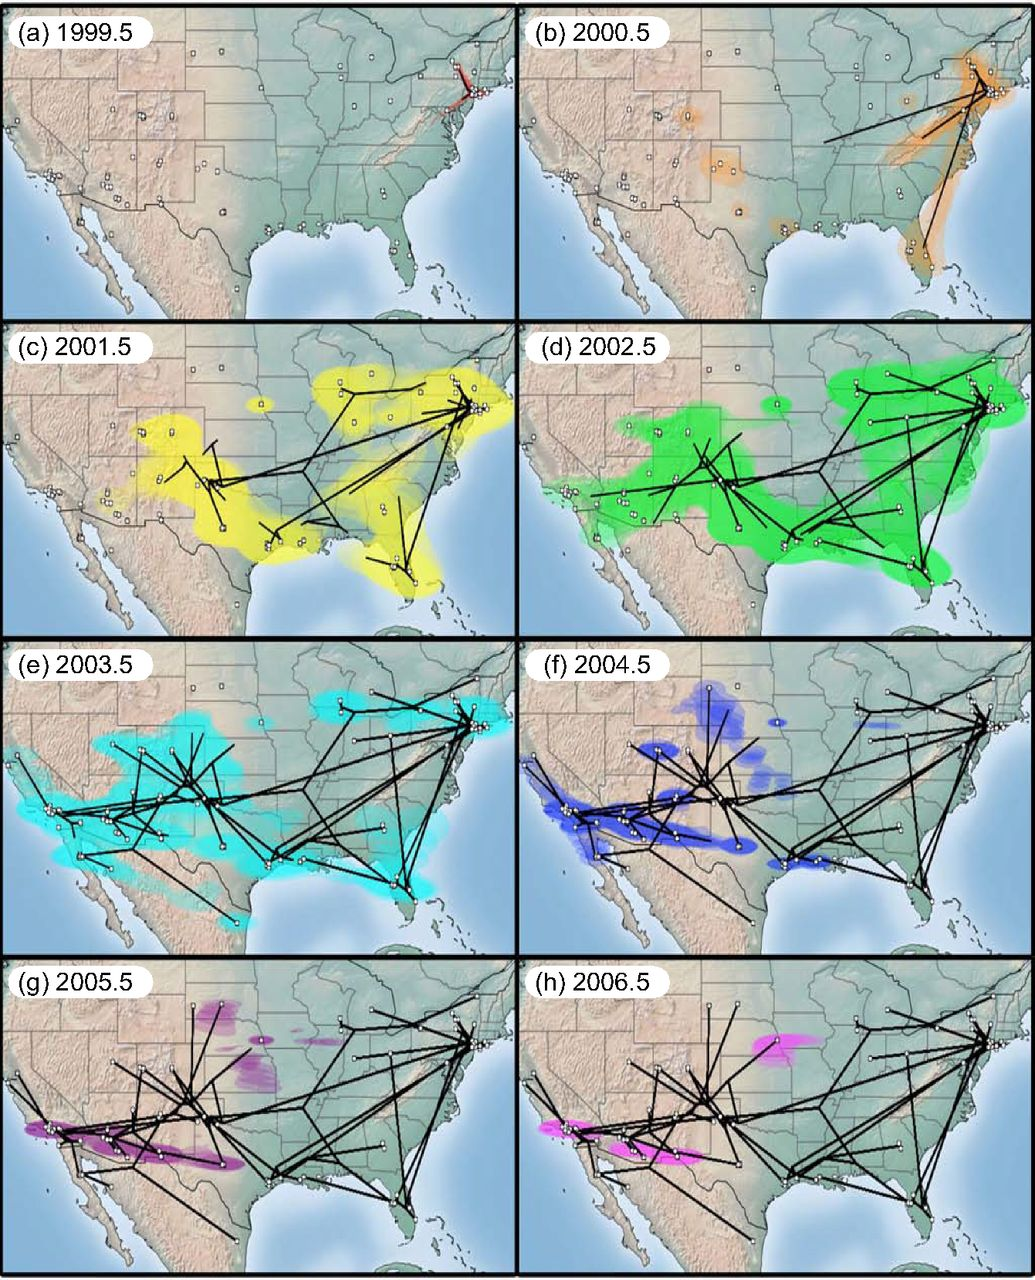
\includegraphics[width=0.5\textwidth]{../images/pybus-fig2.jpg}
%         \caption{\tiny \shortfullcite{Pybus2012}}
%         \end{center}
%     \end{figure}
% \end{frame}

\begin{frame}
    \frametitle{Ebola}
    \begin{adjustwidth}{-1.5em}{-1.5em}
    \begin{figure}
        \begin{center}
        \includegraphics[width=\linewidth]{../images/gire-et-al-2014-ebola-fig3.jpg}
        \caption{\tiny \shortfullcite{Gire2014}}
        \end{center}
    \end{figure}
    \end{adjustwidth}
\end{frame}



% \begin{frame}
% \frametitle{Outline}
% \tableofcontents[currentsection]
% \end{frame}

%%%%%%%%%%%%%%%%%%%%%%%%%%%%%%%%%%%%%%%%%
\subsection{Tree basics}
%%%%%%%%%%%%%%%%%%%%%%%%%%%%%%%%%%%%%%%%%

\tikzset{node lower left/.style={font=\scriptsize,anchor=north east,text height=0.192cm,text depth=0.055cm,inner sep=0.03cm},
leaf/.style={font=\small,anchor=west,text height=0.240cm,text depth=0.068cm},
node upper left/.style={font=\scriptsize,anchor=south east,text height=0.192cm,text depth=0.055cm,inner sep=0.03cm},
bracket label/.style={font=\small,anchor=west,text height=0.240cm,text depth=0.068cm,inner sep=0.1cm},
node upper right/.style={font=\scriptsize,anchor=south west,text height=0.192cm,text depth=0.055cm,inner sep=0.03cm},
node right/.style={font=\scriptsize,anchor=west,text height=0.192cm,text depth=0.055cm,inner sep=0.03cm},
branch/.style={font=\tiny,text height=0.144cm,text depth=0.041cm,inner sep=0.025cm},
root/.style={font=\small,anchor=east,text height=0.240cm,text depth=0.068cm},
node lower right/.style={font=\scriptsize,anchor=north west,text height=0.192cm,text depth=0.055cm,inner sep=0.03cm}}

\begin{frame}
    \frametitle{Tree terminology}

        %% This is a tikz file
\begin{tikzpicture}[scale=1.4,very thick,inner sep=0.1cm]
%        +---3:\hspace{11mm}\includegraphics[height=6.5mm,resolution=150]{../images/Alces.png}
%     +--2
%     |  | +--5:\hspace{11mm}\includegraphics[width=12mm,resolution=150]{../images/Rattus.png}
%     |  +-4
%   +-1    +--6:\hspace{11mm}\includegraphics[height=6.5mm,resolution=150]{../images/Homo-sapiens.png}
%   | |
% 1:0 +------7:\hspace{11mm}\includegraphics[height=6.5mm,resolution=150]{../images/Loxodonta.png}
%   |
%   |      +-9:\hspace{11mm}\includegraphics[height=6.5mm,resolution=150]{../images/Phascolarctos.png}
%   +------8
%          +-10:\hspace{11mm}\includegraphics[height=6.5mm,resolution=150]{../images/Macropus.png}

% The scale is 0.960000, and the yScale is 0.800000

%% Coordinates of nodes.
\coordinate (nr) at (-0.4,1.450);
\coordinate (n0) at (0.000,1.450);
\coordinate (n0ae) at (-0.05,1.4);
\coordinate (n0as) at (-0.4,1.1);
\coordinate (n1) at (0.960,2.500);
\coordinate (n1p) at (0.000,2.500);
\coordinate (n2) at (1.920,3.400);
\coordinate (n2ae) at (1.860,3.450);
\coordinate (n2as) at (1.420,3.750);
\coordinate (n2p) at (0.960,3.400);
\coordinate (n3) at (3.840,4.000);
\coordinate (n3ae) at (3.8,4.06);
\coordinate (n3as) at (3.5,4.4);
\coordinate (n3p) at (1.920,4.000);
\coordinate (n4) at (2.880,2.800);
\coordinate (n4p) at (1.920,2.800);
\coordinate (n5) at (3.840,3.200);
\coordinate (n5p) at (2.880,3.200);
\coordinate (n6) at (3.840,2.400);
\coordinate (n6p) at (2.880,2.400);
\coordinate (n7) at (3.840,1.600);
\coordinate (n7p) at (0.960,1.600);
\coordinate (n8) at (2.880,0.400);
\coordinate (n8ae) at (1.440,0.350);
\coordinate (n8as) at (1.040,0.000);
\coordinate (n8p) at (0.000,0.400);
\coordinate (n9) at (3.840,0.800);
\coordinate (n9p) at (2.880,0.800);
\coordinate (n10) at (3.840,0.000);
\coordinate (n10p) at (2.880,0.000);

%% horizontal lines
\draw (n1p) -- (n1);
\draw (n2p) -- (n2);
\draw (n3p) -- (n3);
\draw (n4p) -- (n4);
\draw (n5p) -- (n5);
\draw (n6p) -- (n6);
\draw (n7p) -- (n7);
\draw (n8p) -- (n8);
\draw (n9p) -- (n9);
\draw (n10p) -- (n10);
\draw (n0) -- (nr);

%% vertical lines
\draw [line cap=rect] (n1p) -- (n8p);
\draw [line cap=rect] (n2p) -- (n7p);
\draw [line cap=rect] (n3p) -- (n4p);
\draw [line cap=rect] (n5p) -- (n6p);
\draw [line cap=rect] (n9p) -- (n10p);

%% arrows
\draw [thick, <-, color=red] (n0ae) -- (n0as) node[align=left, left]{\hmask{\sffamily Root node}};
\draw [thick, <-, color=red] (n3ae) -- (n3as) node[align=left, left]{\hmask{\sffamily Terminal node \\(or leaf, tip)}};
\draw [thick, <-, color=red] (n2ae) -- (n2as) node[align=left, left]{\hmask{\sffamily Internal node}};
\draw [thick, <-, color=red] (n8ae) -- (n8as) node[align=right, left]{\hmask{\sffamily Branch}};

%% leaf labels
\node at (n3)  {\hspace{13mm}\includegraphics[height=8.5mm,resolution=150]{../images/Alces.png}};
\node at (n5)  {\hspace{13mm}\includegraphics[width=14mm,resolution=150]{../images/Rattus.png}};
\node at (n6)  {\hspace{13mm}\includegraphics[height=8.5mm,resolution=150]{../images/Homo-sapiens.png}};
\node at (n7)  {\hspace{13mm}\includegraphics[height=8.5mm,resolution=150]{../images/Loxodonta.png}};
\node at (n9)  {\hspace{13mm}\includegraphics[height=8.5mm,resolution=150]{../images/Phascolarctos.png}};
\node at (n10) {\hspace{13mm}\includegraphics[height=8.5mm,resolution=150]{../images/Macropus.png}};

%% root label
\node [root] at (nr) {};

% internal node labels (doSmartLabels is True)

\end{tikzpicture}


\end{frame}

\tikzset{node lower left/.style={font=\scriptsize,anchor=north east,text height=0.192cm,text depth=0.055cm,inner sep=0.03cm},
leaf/.style={font=\small,anchor=west,text height=0.240cm,text depth=0.068cm},
node upper left/.style={font=\scriptsize,anchor=south east,text height=0.192cm,text depth=0.055cm,inner sep=0.03cm},
bracket label/.style={font=\small,anchor=west,text height=0.240cm,text depth=0.068cm,inner sep=0.1cm},
node upper right/.style={font=\scriptsize,anchor=south west,text height=0.192cm,text depth=0.055cm,inner sep=0.03cm},
node right/.style={font=\scriptsize,anchor=west,text height=0.192cm,text depth=0.055cm,inner sep=0.03cm},
branch/.style={font=\tiny,text height=0.144cm,text depth=0.041cm,inner sep=0.025cm},
root/.style={font=\small,anchor=east,text height=0.240cm,text depth=0.068cm},
node lower right/.style={font=\scriptsize,anchor=north west,text height=0.192cm,text depth=0.055cm,inner sep=0.03cm}}

\clickerslide{
\begin{noheadline}
\begin{frame}
    \begin{adjustwidth}{-1.5em}{-1.5em}
    \begin{clickerquestion}
        \item Three of these trees describe the same relationships. Which one
            is different?
    \end{clickerquestion}
    % \vspace{-0.5cm}
    \begin{columns}

        \column{0.5\linewidth}

        %% This is a tikz file
\begin{tikzpicture}[very thick,inner sep=0.1cm]
%        +---3:\hspace{11mm}\includegraphics[height=6.5mm,resolution=150]{../images/Alces.png}
%     +--2
%     |  | +--5:\hspace{11mm}\includegraphics[width=12mm,resolution=150]{../images/Rattus.png}
%     |  +-4
%   +-1    +--6:\hspace{11mm}\includegraphics[height=6.5mm,resolution=150]{../images/Homo-sapiens.png}
%   | |
% 1:0 +------7:\hspace{11mm}\includegraphics[height=6.5mm,resolution=150]{../images/Loxodonta.png}
%   |
%   |      +-9:\hspace{11mm}\includegraphics[height=6.5mm,resolution=150]{../images/Phascolarctos.png}
%   +------8
%          +-10:\hspace{11mm}\includegraphics[height=6.5mm,resolution=150]{../images/Macropus.png}

% The scale is 0.960000, and the yScale is 0.800000

%% Coordinates of nodes.
\coordinate (nr) at (-0.4,1.450);
\coordinate (n0) at (0.000,1.450);
\coordinate (n1) at (0.960,2.500);
\coordinate (n1p) at (0.000,2.500);
\coordinate (n2) at (1.920,3.400);
\coordinate (n2p) at (0.960,3.400);
\coordinate (n3) at (3.840,4.000);
\coordinate (n3p) at (1.920,4.000);
\coordinate (n4) at (2.880,2.800);
\coordinate (n4p) at (1.920,2.800);
\coordinate (n5) at (3.840,3.200);
\coordinate (n5p) at (2.880,3.200);
\coordinate (n6) at (3.840,2.400);
\coordinate (n6p) at (2.880,2.400);
\coordinate (n7) at (3.840,1.600);
\coordinate (n7p) at (0.960,1.600);
\coordinate (n8) at (2.880,0.400);
\coordinate (n8p) at (0.000,0.400);
\coordinate (n9) at (3.840,0.800);
\coordinate (n9p) at (2.880,0.800);
\coordinate (n10) at (3.840,0.000);
\coordinate (n10p) at (2.880,0.000);

%% horizontal lines
\draw (n1p) -- (n1);
\draw (n2p) -- (n2);
\draw (n3p) -- (n3);
\draw (n4p) -- (n4);
\draw (n5p) -- (n5);
\draw (n6p) -- (n6);
\draw (n7p) -- (n7);
\draw (n8p) -- (n8);
\draw (n9p) -- (n9);
\draw (n10p) -- (n10);
\draw (n0) -- (nr);

%% vertical lines
\draw [line cap=rect] (n1p) -- (n8p);
\draw [line cap=rect] (n2p) -- (n7p);
\draw [line cap=rect] (n3p) -- (n4p);
\draw [line cap=rect] (n5p) -- (n6p);
\draw [line cap=rect] (n9p) -- (n10p);

%% leaf labels
\node at (n3) {\hspace{11mm}\includegraphics[height=6.5mm,resolution=150]{../images/Alces.png}};
\node at (n5) {\hspace{11mm}\includegraphics[width=12mm,resolution=150]{../images/Rattus.png}};
\node at (n6) {\hspace{11mm}\includegraphics[height=6.5mm,resolution=150]{../images/Homo-sapiens.png}};
\node at (n7) {\hspace{11mm}\includegraphics[height=6.5mm,resolution=150]{../images/Loxodonta.png}};
\node at (n9) {\hspace{11mm}\includegraphics[height=6.5mm,resolution=150]{../images/Phascolarctos.png}};
\node at (n10) {\hspace{11mm}\includegraphics[height=6.5mm,resolution=150]{../images/Macropus.png}};

%% root label
\node [root] at (nr) {\textcolor{red}{\sffamily\LARGE\bf 1)}};

% internal node labels (doSmartLabels is True)

\end{tikzpicture}


        % \vspace{-1cm}

        %% This is a tikz file
\begin{tikzpicture}[very thick,inner sep=0.1cm]
%     +-----2:\hspace{11mm}\includegraphics[height=6.5mm,resolution=150]{../images/Loxodonta.png}
%     |
%   +-1    +-5:\hspace{11mm}\includegraphics[width=12mm,resolution=150]{../images/Rattus.png}
%   | | +--4
%   | +-3  +-6:\hspace{11mm}\includegraphics[height=6.5mm,resolution=150]{../images/Homo-sapiens.png}
%   |   |
% 3:0   +---7:\hspace{11mm}\includegraphics[height=6.5mm,resolution=150]{../images/Alces.png}
%   |
%   |     +-9:\hspace{11mm}\includegraphics[height=6.5mm,resolution=150]{../images/Macropus.png}
%   +-----8
%         +-10:\hspace{11mm}\includegraphics[height=6.5mm,resolution=150]{../images/Phascolarctos.png}

% The scale is 0.960000, and the yScale is 0.800000

%% Coordinates of nodes.
\coordinate (nr) at (-0.4,1.750);
\coordinate (n0) at (0.000,1.750);
\coordinate (n1) at (0.960,3.100);
\coordinate (n1p) at (0.000,3.100);
\coordinate (n2) at (3.840,4.000);
\coordinate (n2p) at (0.960,4.000);
\coordinate (n3) at (1.920,2.200);
\coordinate (n3p) at (0.960,2.200);
\coordinate (n4) at (2.880,2.800);
\coordinate (n4p) at (1.920,2.800);
\coordinate (n5) at (3.840,3.200);
\coordinate (n5p) at (2.880,3.200);
\coordinate (n6) at (3.840,2.400);
\coordinate (n6p) at (2.880,2.400);
\coordinate (n7) at (3.840,1.600);
\coordinate (n7p) at (1.920,1.600);
\coordinate (n8) at (2.880,0.400);
\coordinate (n8p) at (0.000,0.400);
\coordinate (n9) at (3.840,0.800);
\coordinate (n9p) at (2.880,0.800);
\coordinate (n10) at (3.840,0.000);
\coordinate (n10p) at (2.880,0.000);

%% horizontal lines
\draw (n1p) -- (n1);
\draw (n2p) -- (n2);
\draw (n3p) -- (n3);
\draw (n4p) -- (n4);
\draw (n5p) -- (n5);
\draw (n6p) -- (n6);
\draw (n7p) -- (n7);
\draw (n8p) -- (n8);
\draw (n9p) -- (n9);
\draw (n10p) -- (n10);
\draw (n0) -- (nr);

%% vertical lines
\draw [line cap=rect] (n1p) -- (n8p);
\draw [line cap=rect] (n2p) -- (n3p);
\draw [line cap=rect] (n4p) -- (n7p);
\draw [line cap=rect] (n5p) -- (n6p);
\draw [line cap=rect] (n9p) -- (n10p);

%% leaf labels
\node at (n2) {\hspace{11mm}\includegraphics[height=6.5mm,resolution=150]{../images/Loxodonta.png}};
\node at (n5) {\hspace{11mm}\includegraphics[width=12mm,resolution=150]{../images/Rattus.png}};
\node at (n6) {\hspace{11mm}\includegraphics[height=6.5mm,resolution=150]{../images/Homo-sapiens.png}};
\node at (n7) {\hspace{11mm}\includegraphics[height=6.5mm,resolution=150]{../images/Alces.png}};
\node at (n9) {\hspace{11mm}\includegraphics[height=6.5mm,resolution=150]{../images/Macropus.png}};
\node at (n10) {\hspace{11mm}\includegraphics[height=6.5mm,resolution=150]{../images/Phascolarctos.png}};

%% root label
\node [root] at (nr) {\textcolor{red}{\sffamily\LARGE\bf 3)}};

% internal node labels (doSmartLabels is True)

\end{tikzpicture}


        \column{0.5\linewidth}

        %% This is a tikz file
\begin{tikzpicture}[scale=0.8,very thick,inner sep=0.1cm]
%         +-2:\hspace{11mm}\includegraphics[height=6.5mm,resolution=150]{../images/Phascolarctos.png}
%   +-----1
%   |     +-3:\hspace{11mm}\includegraphics[height=6.5mm,resolution=150]{../images/Macropus.png}
% 2:0
%   | +-----5:\hspace{11mm}\includegraphics[height=6.5mm,resolution=150]{../images/Loxodonta.png}
%   | |
%   +-4 +----7:\hspace{11mm}\includegraphics[height=6.5mm,resolution=150]{../images/Alces.png}
%     +-6
%       |  +-9:\hspace{11mm}\includegraphics[width=12mm,resolution=150]{../images/Rattus.png}
%       +--8
%          +-10:\hspace{11mm}\includegraphics[height=6.5mm,resolution=150]{../images/Homo-sapiens.png}

% The scale is 0.960000, and the yScale is 0.800000

%% Coordinates of nodes.
\coordinate (nr) at (-0.4,2.650);
\coordinate (n0) at (0.000,2.650);
\coordinate (n1) at (2.880,3.600);
\coordinate (n1p) at (0.000,3.600);
\coordinate (n2) at (3.840,4.000);
\coordinate (n2p) at (2.880,4.000);
\coordinate (n3) at (3.840,3.200);
\coordinate (n3p) at (2.880,3.200);
\coordinate (n4) at (0.960,1.700);
\coordinate (n4p) at (0.000,1.700);
\coordinate (n5) at (3.840,2.400);
\coordinate (n5p) at (0.960,2.400);
\coordinate (n6) at (1.920,1.000);
\coordinate (n6p) at (0.960,1.000);
\coordinate (n7) at (3.840,1.600);
\coordinate (n7p) at (1.920,1.600);
\coordinate (n8) at (2.880,0.400);
\coordinate (n8p) at (1.920,0.400);
\coordinate (n9) at (3.840,0.800);
\coordinate (n9p) at (2.880,0.800);
\coordinate (n10) at (3.840,0.000);
\coordinate (n10p) at (2.880,0.000);

%% horizontal lines
\draw (n1p) -- (n1);
\draw (n2p) -- (n2);
\draw (n3p) -- (n3);
\draw (n4p) -- (n4);
\draw (n5p) -- (n5);
\draw (n6p) -- (n6);
\draw (n7p) -- (n7);
\draw (n8p) -- (n8);
\draw (n9p) -- (n9);
\draw (n10p) -- (n10);
\draw (n0) -- (nr);

%% vertical lines
\draw [line cap=rect] (n1p) -- (n4p);
\draw [line cap=rect] (n2p) -- (n3p);
\draw [line cap=rect] (n5p) -- (n6p);
\draw [line cap=rect] (n7p) -- (n8p);
\draw [line cap=rect] (n9p) -- (n10p);

%% leaf labels
\node at (n2)  {\hspace{11mm}\includegraphics[height=5.5mm,resolution=150]{../images/Phascolarctos.png}};
\node at (n3)  {\hspace{11mm}\includegraphics[height=5.5mm,resolution=150]{../images/Macropus.png}};
\node at (n5)  {\hspace{11mm}\includegraphics[height=5.5mm,resolution=150]{../images/Loxodonta.png}};
\node at (n7)  {\hspace{11mm}\includegraphics[height=5.5mm,resolution=150]{../images/Alces.png}};
\node at (n9)  {\hspace{11mm}\includegraphics[width=11mm,resolution=150]{../images/Rattus.png}};
\node at (n10) {\hspace{11mm}\includegraphics[height=5.5mm,resolution=150]{../images/Homo-sapiens.png}};

%% root label
\node [root] at (nr) {\textcolor{red}{\sffamily\LARGE\bf 2)}};

% internal node labels (doSmartLabels is True)

\end{tikzpicture}


        % \vspace{-1cm}

        %% This is a tikz file
\begin{tikzpicture}[scale=0.8,very thick,inner sep=0.1cm]
%     +------2:\hspace{11mm}\includegraphics[height=6.5mm,resolution=150]{../images/Alces.png}
%     |
%   +-1    +--5:\hspace{11mm}\includegraphics[width=12mm,resolution=150]{../images/Rattus.png}
%   | |  +-4
%   | +--3 +--6:\hspace{11mm}\includegraphics[height=6.5mm,resolution=150]{../images/Homo-sapiens.png}
%   |    |
% 4:0    +---7:\hspace{11mm}\includegraphics[height=6.5mm,resolution=150]{../images/Loxodonta.png}
%   |
%   |      +-9:\hspace{11mm}\includegraphics[height=6.5mm,resolution=150]{../images/Phascolarctos.png}
%   +------8
%          +-10:\hspace{11mm}\includegraphics[height=6.5mm,resolution=150]{../images/Macropus.png}

% The scale is 0.960000, and the yScale is 0.800000

%% Coordinates of nodes.
\coordinate (nr) at (-0.4,1.750);
\coordinate (n0) at (0.000,1.750);
\coordinate (n1) at (0.960,3.100);
\coordinate (n1p) at (0.000,3.100);
\coordinate (n2) at (3.840,4.000);
\coordinate (n2p) at (0.960,4.000);
\coordinate (n3) at (1.920,2.200);
\coordinate (n3p) at (0.960,2.200);
\coordinate (n4) at (2.880,2.800);
\coordinate (n4p) at (1.920,2.800);
\coordinate (n5) at (3.840,3.200);
\coordinate (n5p) at (2.880,3.200);
\coordinate (n6) at (3.840,2.400);
\coordinate (n6p) at (2.880,2.400);
\coordinate (n7) at (3.840,1.600);
\coordinate (n7p) at (1.920,1.600);
\coordinate (n8) at (2.880,0.400);
\coordinate (n8p) at (0.000,0.400);
\coordinate (n9) at (3.840,0.800);
\coordinate (n9p) at (2.880,0.800);
\coordinate (n10) at (3.840,0.000);
\coordinate (n10p) at (2.880,0.000);

%% horizontal lines
\draw (n1p) -- (n1);
\draw (n2p) -- (n2);
\draw (n3p) -- (n3);
\draw (n4p) -- (n4);
\draw (n5p) -- (n5);
\draw (n6p) -- (n6);
\draw (n7p) -- (n7);
\draw (n8p) -- (n8);
\draw (n9p) -- (n9);
\draw (n10p) -- (n10);
\draw (n0) -- (nr);

%% vertical lines
\draw [line cap=rect] (n1p) -- (n8p);
\draw [line cap=rect] (n2p) -- (n3p);
\draw [line cap=rect] (n4p) -- (n7p);
\draw [line cap=rect] (n5p) -- (n6p);
\draw [line cap=rect] (n9p) -- (n10p);

%% leaf labels
\node at (n2)  {\hspace{11mm}\includegraphics[height=5.5mm,resolution=150]{../images/Alces.png}};
\node at (n5)  {\hspace{11mm}\includegraphics[width=11mm,resolution=150]{../images/Rattus.png}};
\node at (n6)  {\hspace{11mm}\includegraphics[height=5.5mm,resolution=150]{../images/Homo-sapiens.png}};
\node at (n7)  {\hspace{11mm}\includegraphics[height=5.5mm,resolution=150]{../images/Loxodonta.png}};
\node at (n9)  {\hspace{11mm}\includegraphics[height=5.5mm,resolution=150]{../images/Phascolarctos.png}};
\node at (n10) {\hspace{11mm}\includegraphics[height=5.5mm,resolution=150]{../images/Macropus.png}};

%% root label
\node [root] at (nr) {\textcolor{red}{\sffamily\LARGE\bf 4)}};

% internal node labels (doSmartLabels is True)

\end{tikzpicture}

        
    \end{columns}
    \end{adjustwidth}
\end{frame}
\end{noheadline}
}




\begin{noheadline}
\begin{frame}
    \begin{adjustwidth}{-1.5em}{-1.5em}
    \textbf{Monophyletic group} =  A group that consists of an ancestor and all
    of its descendants. Circle a monophyletic group on this tree:

    \begin{center}
        %% This is a tikz file
\begin{tikzpicture}[scale=1.4,very thick,inner sep=0.1cm]
%        +---3:\hspace{11mm}\includegraphics[height=6.5mm,resolution=150]{../images/Alces.png}
%     +--2
%     |  | +--5:\hspace{11mm}\includegraphics[width=12mm,resolution=150]{../images/Rattus.png}
%     |  +-4
%   +-1    +--6:\hspace{11mm}\includegraphics[height=6.5mm,resolution=150]{../images/Homo-sapiens.png}
%   | |
% 1:0 +------7:\hspace{11mm}\includegraphics[height=6.5mm,resolution=150]{../images/Loxodonta.png}
%   |
%   |      +-9:\hspace{11mm}\includegraphics[height=6.5mm,resolution=150]{../images/Phascolarctos.png}
%   +------8
%          +-10:\hspace{11mm}\includegraphics[height=6.5mm,resolution=150]{../images/Macropus.png}

% The scale is 0.960000, and the yScale is 0.800000

%% Coordinates of nodes.
\coordinate (nr) at (-0.4,1.450);
\coordinate (n0) at (0.000,1.450);
\coordinate (n0ae) at (-0.05,1.4);
\coordinate (n0as) at (-0.4,1.1);
\coordinate (n1) at (0.960,2.500);
\coordinate (n1p) at (0.000,2.500);
\coordinate (n2) at (1.920,3.400);
\coordinate (n2ae) at (1.860,3.450);
\coordinate (n2as) at (1.420,3.750);
\coordinate (n2p) at (0.960,3.400);
\coordinate (n3) at (3.840,4.000);
\coordinate (n3ae) at (3.8,4.06);
\coordinate (n3as) at (3.5,4.4);
\coordinate (n3p) at (1.920,4.000);
\coordinate (n4) at (2.880,2.800);
\coordinate (n4p) at (1.920,2.800);
\coordinate (n5) at (3.840,3.200);
\coordinate (n5p) at (2.880,3.200);
\coordinate (n6) at (3.840,2.400);
\coordinate (n6p) at (2.880,2.400);
\coordinate (n7) at (3.840,1.600);
\coordinate (n7p) at (0.960,1.600);
\coordinate (n8) at (2.880,0.400);
\coordinate (n8ae) at (1.440,0.350);
\coordinate (n8as) at (1.040,0.000);
\coordinate (n8p) at (0.000,0.400);
\coordinate (n9) at (3.840,0.800);
\coordinate (n9p) at (2.880,0.800);
\coordinate (n10) at (3.840,0.000);
\coordinate (n10p) at (2.880,0.000);

%% horizontal lines
\draw (n1p) -- (n1);
\draw (n2p) -- (n2);
\draw (n3p) -- (n3);
\draw (n4p) -- (n4);
\draw (n5p) -- (n5);
\draw (n6p) -- (n6);
\draw (n7p) -- (n7);
\draw (n8p) -- (n8);
\draw (n9p) -- (n9);
\draw (n10p) -- (n10);
\draw (n0) -- (nr);

%% vertical lines
\draw [line cap=rect] (n1p) -- (n8p);
\draw [line cap=rect] (n2p) -- (n7p);
\draw [line cap=rect] (n3p) -- (n4p);
\draw [line cap=rect] (n5p) -- (n6p);
\draw [line cap=rect] (n9p) -- (n10p);

%% arrows
% \draw [thick, <-, color=red] (n0ae) -- (n0as) node[align=left, left]{\hmask{\sffamily Root node}};
% \draw [thick, <-, color=red] (n3ae) -- (n3as) node[align=left, left]{\hmask{\sffamily Terminal node \\(or leaf, tip)}};
% \draw [thick, <-, color=red] (n2ae) -- (n2as) node[align=left, left]{\hmask{\sffamily Internal node}};
% \draw [thick, <-, color=red] (n8ae) -- (n8as) node[align=right, left]{\hmask{\sffamily Branch}};

%% leaf labels
\node at (n3)  {\hspace{13mm}\includegraphics[height=8.5mm,resolution=150]{../images/Alces.png}};
\node at (n5)  {\hspace{13mm}\includegraphics[width=14mm,resolution=150]{../images/Rattus.png}};
\node at (n6)  {\hspace{13mm}\includegraphics[height=8.5mm,resolution=150]{../images/Homo-sapiens.png}};
\node at (n7)  {\hspace{13mm}\includegraphics[height=8.5mm,resolution=150]{../images/Loxodonta.png}};
\node at (n9)  {\hspace{13mm}\includegraphics[height=8.5mm,resolution=150]{../images/Phascolarctos.png}};
\node at (n10) {\hspace{13mm}\includegraphics[height=8.5mm,resolution=150]{../images/Macropus.png}};

%% root label
\node [root] at (nr) {};

% internal node labels (doSmartLabels is True)

\end{tikzpicture}

    \end{center}

    \end{adjustwidth}
\end{frame}
\end{noheadline}


\clickerslide{
\begin{noheadline}
\begin{frame}[t]
    \begin{adjustwidth}{-1.5em}{-1.5em}
        \vspace{-3.5mm}
    \begin{clickerquestion}
        \item In reference to the phylogeny below, which of the following
            statements are correct?
            \vspace{-0.5mm}
        \begin{clickeroptions}
            % \begin{columns}
                \small
                % \column{0.82\linewidth}
            \item Elephants, humans, and rats are NOT monophyletic.
            \item Moose, humans, and rats are monophyletic.
            \item Elephants are more closely related to moose
                    than koalas.
            \item Moose are more closely related to humans than elephants.
                % \column{0.2\linewidth}
            \item None of the above.
            \item \clickeranswer{Answers 1, 2, 3, \& 4.}
            % \end{columns}
        \end{clickeroptions}
    \end{clickerquestion}

    \vspace{-8mm}
    \begin{center}
        %% This is a tikz file
\begin{tikzpicture}[scale=1.4,very thick,inner sep=0.1cm]
%        +---3:\hspace{11mm}\includegraphics[height=6.5mm,resolution=150]{../images/Alces.png}
%     +--2
%     |  | +--5:\hspace{11mm}\includegraphics[width=12mm,resolution=150]{../images/Rattus.png}
%     |  +-4
%   +-1    +--6:\hspace{11mm}\includegraphics[height=6.5mm,resolution=150]{../images/Homo-sapiens.png}
%   | |
% 1:0 +------7:\hspace{11mm}\includegraphics[height=6.5mm,resolution=150]{../images/Loxodonta.png}
%   |
%   |      +-9:\hspace{11mm}\includegraphics[height=6.5mm,resolution=150]{../images/Phascolarctos.png}
%   +------8
%          +-10:\hspace{11mm}\includegraphics[height=6.5mm,resolution=150]{../images/Macropus.png}

% The scale is 0.960000, and the yScale is 0.800000

%% Coordinates of nodes.
\coordinate (nr) at (-0.4,1.450);
\coordinate (n0) at (0.000,1.450);
\coordinate (n0ae) at (-0.05,1.4);
\coordinate (n0as) at (-0.4,1.1);
\coordinate (n1) at (0.960,2.500);
\coordinate (n1p) at (0.000,2.500);
\coordinate (n2) at (1.920,3.400);
\coordinate (n2ae) at (1.860,3.450);
\coordinate (n2as) at (1.420,3.750);
\coordinate (n2p) at (0.960,3.400);
\coordinate (n3) at (3.840,4.000);
\coordinate (n3ae) at (3.8,4.06);
\coordinate (n3as) at (3.5,4.4);
\coordinate (n3p) at (1.920,4.000);
\coordinate (n4) at (2.880,2.800);
\coordinate (n4p) at (1.920,2.800);
\coordinate (n5) at (3.840,3.200);
\coordinate (n5p) at (2.880,3.200);
\coordinate (n6) at (3.840,2.400);
\coordinate (n6p) at (2.880,2.400);
\coordinate (n7) at (3.840,1.600);
\coordinate (n7p) at (0.960,1.600);
\coordinate (n8) at (2.880,0.400);
\coordinate (n8ae) at (1.440,0.350);
\coordinate (n8as) at (1.040,0.000);
\coordinate (n8p) at (0.000,0.400);
\coordinate (n9) at (3.840,0.800);
\coordinate (n9p) at (2.880,0.800);
\coordinate (n10) at (3.840,0.000);
\coordinate (n10p) at (2.880,0.000);

%% horizontal lines
\draw (n1p) -- (n1);
\draw (n2p) -- (n2);
\draw (n3p) -- (n3);
\draw (n4p) -- (n4);
\draw (n5p) -- (n5);
\draw (n6p) -- (n6);
\draw (n7p) -- (n7);
\draw (n8p) -- (n8);
\draw (n9p) -- (n9);
\draw (n10p) -- (n10);
\draw (n0) -- (nr);

%% vertical lines
\draw [line cap=rect] (n1p) -- (n8p);
\draw [line cap=rect] (n2p) -- (n7p);
\draw [line cap=rect] (n3p) -- (n4p);
\draw [line cap=rect] (n5p) -- (n6p);
\draw [line cap=rect] (n9p) -- (n10p);

%% arrows
% \draw [thick, <-, color=red] (n0ae) -- (n0as) node[align=left, left]{\hmask{\sffamily Root node}};
% \draw [thick, <-, color=red] (n3ae) -- (n3as) node[align=left, left]{\hmask{\sffamily Terminal node \\(or leaf, tip)}};
% \draw [thick, <-, color=red] (n2ae) -- (n2as) node[align=left, left]{\hmask{\sffamily Internal node}};
% \draw [thick, <-, color=red] (n8ae) -- (n8as) node[align=right, left]{\hmask{\sffamily Branch}};

%% leaf labels
\node at (n3)  {\hspace{13mm}\includegraphics[height=8.5mm,resolution=150]{../images/Alces.png}};
\node at (n5)  {\hspace{13mm}\includegraphics[width=14mm,resolution=150]{../images/Rattus.png}};
\node at (n6)  {\hspace{13mm}\includegraphics[height=8.5mm,resolution=150]{../images/Homo-sapiens.png}};
\node at (n7)  {\hspace{13mm}\includegraphics[height=8.5mm,resolution=150]{../images/Loxodonta.png}};
\node at (n9)  {\hspace{13mm}\includegraphics[height=8.5mm,resolution=150]{../images/Phascolarctos.png}};
\node at (n10) {\hspace{13mm}\includegraphics[height=8.5mm,resolution=150]{../images/Macropus.png}};

%% root label
\node [root] at (nr) {};

% internal node labels (doSmartLabels is True)

\end{tikzpicture}

    \end{center}

    \end{adjustwidth}
\end{frame}
\end{noheadline}
}

\begin{noheadline}
\begin{frame}
    \begin{adjustwidth}{-1.5em}{-1.5em}
        \begin{itemize}
            \item Marsupials, like kangaroos and koalas, raise their young in a
                pouch.  Draw on the tree below where pouches evolved.

            \item Stegodons had trunks (highly modified noses); add stegodons
                to the tree and label where trunks evolved.
        \end{itemize}

    \begin{center}
        %% This is a tikz file
\begin{tikzpicture}[scale=1.4,very thick,inner sep=0.1cm]
%        +---3:\hspace{11mm}\includegraphics[height=6.5mm,resolution=150]{../images/Alces.png}
%     +--2
%     |  | +--5:\hspace{11mm}\includegraphics[width=12mm,resolution=150]{../images/Rattus.png}
%     |  +-4
%   +-1    +--6:\hspace{11mm}\includegraphics[height=6.5mm,resolution=150]{../images/Homo-sapiens.png}
%   | |
% 1:0 +------7:\hspace{11mm}\includegraphics[height=6.5mm,resolution=150]{../images/Loxodonta.png}
%   |
%   |      +-9:\hspace{11mm}\includegraphics[height=6.5mm,resolution=150]{../images/Phascolarctos.png}
%   +------8
%          +-10:\hspace{11mm}\includegraphics[height=6.5mm,resolution=150]{../images/Macropus.png}

% The scale is 0.960000, and the yScale is 0.800000

%% Coordinates of nodes.
\coordinate (nr) at (-0.4,1.450);
\coordinate (n0) at (0.000,1.450);
\coordinate (n0ae) at (-0.05,1.4);
\coordinate (n0as) at (-0.4,1.1);
\coordinate (n1) at (0.960,2.500);
\coordinate (n1p) at (0.000,2.500);
\coordinate (n2) at (1.920,3.400);
\coordinate (n2ae) at (1.860,3.450);
\coordinate (n2as) at (1.420,3.750);
\coordinate (n2p) at (0.960,3.400);
\coordinate (n3) at (3.840,4.000);
\coordinate (n3ae) at (3.8,4.06);
\coordinate (n3as) at (3.5,4.4);
\coordinate (n3p) at (1.920,4.000);
\coordinate (n4) at (2.880,2.800);
\coordinate (n4p) at (1.920,2.800);
\coordinate (n5) at (3.840,3.200);
\coordinate (n5p) at (2.880,3.200);
\coordinate (n6) at (3.840,2.400);
\coordinate (n6p) at (2.880,2.400);
\coordinate (n7) at (3.840,1.600);
\coordinate (n7p) at (0.960,1.600);
\coordinate (n8) at (2.880,0.400);
\coordinate (n8ae) at (1.440,0.350);
\coordinate (n8as) at (1.040,0.000);
\coordinate (n8p) at (0.000,0.400);
\coordinate (n9) at (3.840,0.800);
\coordinate (n9p) at (2.880,0.800);
\coordinate (n10) at (3.840,0.000);
\coordinate (n10p) at (2.880,0.000);

%% horizontal lines
\draw (n1p) -- (n1);
\draw (n2p) -- (n2);
\draw (n3p) -- (n3);
\draw (n4p) -- (n4);
\draw (n5p) -- (n5);
\draw (n6p) -- (n6);
\draw (n7p) -- (n7);
\draw (n8p) -- (n8);
\draw (n9p) -- (n9);
\draw (n10p) -- (n10);
\draw (n0) -- (nr);

%% vertical lines
\draw [line cap=rect] (n1p) -- (n8p);
\draw [line cap=rect] (n2p) -- (n7p);
\draw [line cap=rect] (n3p) -- (n4p);
\draw [line cap=rect] (n5p) -- (n6p);
\draw [line cap=rect] (n9p) -- (n10p);

%% arrows
% \draw [thick, <-, color=red] (n0ae) -- (n0as) node[align=left, left]{\hmask{\sffamily Root node}};
% \draw [thick, <-, color=red] (n3ae) -- (n3as) node[align=left, left]{\hmask{\sffamily Terminal node \\(or leaf, tip)}};
% \draw [thick, <-, color=red] (n2ae) -- (n2as) node[align=left, left]{\hmask{\sffamily Internal node}};
% \draw [thick, <-, color=red] (n8ae) -- (n8as) node[align=right, left]{\hmask{\sffamily Branch}};

%% leaf labels
\node at (n3)  {\hspace{13mm}\includegraphics[height=8.5mm,resolution=150]{../images/Alces.png}};
\node at (n5)  {\hspace{13mm}\includegraphics[width=14mm,resolution=150]{../images/Rattus.png}};
\node at (n6)  {\hspace{13mm}\includegraphics[height=8.5mm,resolution=150]{../images/Homo-sapiens.png}};
\node at (n7)  {\hspace{13mm}\includegraphics[height=8.5mm,resolution=150]{../images/Loxodonta.png}};
\node at (n9)  {\hspace{13mm}\includegraphics[height=8.5mm,resolution=150]{../images/Phascolarctos.png}};
\node at (n10) {\hspace{13mm}\includegraphics[height=8.5mm,resolution=150]{../images/Macropus.png}};

%% root label
\node [root] at (nr) {};

% internal node labels (doSmartLabels is True)

\end{tikzpicture}

    \end{center}

    \end{adjustwidth}
    \note[item]{Define synapomorphy: A shared derived trait; a trait that is
        unique to a monophyletic group.}
\end{frame}
\end{noheadline}

%%%%%%%%%%%%%%%%%%%%%%%%%%%%%%%%%%%%%%%%%%%%%%%%%%%
\section{Building trees tutorial}
%%%%%%%%%%%%%%%%%%%%%%%%%%%%%%%%%%%%%%%%%%%%%%%%%%%

\begin{frame}
    \frametitle{Phylogenetic trees tutorial}

    \vspace{1cm}
    Work in teams of 3. Middle person as the scribe (does the writing). As you
    work through the questions, be sure to explain your logic to each other.

    \vspace{1cm}
    When you finish the first page, please press "1" on your clickers.

    \vspace{1cm}
    Please ask us for help, if you need it!
\end{frame}

% \begin{frame}[t]
%     \begin{adjustwidth}{-1.5em}{-1.5em}
%     \begin{enumerate}%[Q 1:]
%         \vspace{-2mm}
%         \begin{columns}
%             \small
%             \column{0.7\textwidth}

%             \column{0.3\textwidth}
%             Sharks and rays

%             \vspace{0.6cm}
%             Lizards

%             \vspace{0.6cm}
%             Snakes

%             \vspace{0.6cm}
%             Mammals

%             \vspace{0.6cm}
%             Amphibians

%             \vspace{0.6cm}
%             Ray-finned fish
%         \end{columns}

%             \vspace{0.2cm}
%         \item[Q 5.] Are lizards or sharks more closely related to amphibians?

%             \vspace{0.5cm}
%         \item[Q 6.] Are lizards or ray-finned fish more closely related to sharks?
        
%     \end{enumerate}
%     \end{adjustwidth}
% \end{frame}

\begin{noheadline}
\begin{frame}
    \begin{adjustwidth}{-1.5em}{-1.5em}
        \begin{columns}
            \column{0.3\linewidth}

            Phylogeny of mammals estimated from DNA sequence data

            \column{0.75\linewidth}

            \includegraphics[width=1.02\columnwidth]{mammal-tree.png}

        \end{columns}

    \end{adjustwidth}
\end{frame}
\end{noheadline}

\clickerslide{
\begin{noheadline}
\begin{frame}
    \begin{adjustwidth}{-1.5em}{-1.5em}
        \begin{columns}
            \column{0.3\linewidth}

            \begin{clickerquestion}
                \item From the common ancestor of all mammals, which have been
                    evolving for a longer period of time?
                \begin{clickeroptions}
                    \item Today's monotremes
                    \item Today's bats
                    \item \clickeranswer{Neither (same)}
                \end{clickeroptions}
            \end{clickerquestion}

            \column{0.75\linewidth}

            \includegraphics[width=1.02\columnwidth]{mammal-tree.png}

        \end{columns}

    \end{adjustwidth}
\end{frame}
\end{noheadline}
}

\clickerslide{
\begin{noheadline}
\begin{frame}
    \begin{adjustwidth}{-1.5em}{-1.5em}
        \begin{columns}
            \column{0.3\linewidth}

            \begin{clickerquestion}
                \item Which group is more closely related to apes?
                \begin{clickeroptions}
                    \item Anteaters
                    \item \clickeranswer{Pangolin}
                    \item Neither (same)
                \end{clickeroptions}
            \end{clickerquestion}

            \column{0.75\linewidth}

            \includegraphics[width=1.02\columnwidth]{mammal-tree.png}

        \end{columns}

    \end{adjustwidth}

    \note[item]{This is the same as asking which group has the most recent
        common ancestor with apes}
\end{frame}
\end{noheadline}
}

\clickerslide{
\begin{noheadline}
\begin{frame}
    \begin{adjustwidth}{-1.5em}{-1.5em}
        \begin{columns}
            \column{0.3\linewidth}

            \begin{clickerquestion}
                \item Was the common ancestor of pangolins and apes a pangolin,
                    or an ape?
                \begin{clickeroptions}
                    \item Ape 
                    \item Pangolin
                    \item \clickeranswer{Neither (different)}
                \end{clickeroptions}
            \end{clickerquestion}

            \column{0.75\linewidth}

            \includegraphics[width=1.02\columnwidth]{mammal-tree.png}

        \end{columns}

    \end{adjustwidth}

    \note[item]{Pangolins and apes are derived from a common ancestor that was
        different from either of them.}
\end{frame}
\end{noheadline}
}

\clickerslide{
\begin{noheadline}
\begin{frame}
    \begin{adjustwidth}{-1.5em}{-1.5em}
        \begin{columns}
            \column{0.3\linewidth}

            \begin{clickerquestion}
                \item Which group is more closely related to anteaters?
                \begin{clickeroptions}
                    \item Apes
                    \item Pangolin
                    \item \clickeranswer{Neither (same)}
                \end{clickeroptions}
            \end{clickerquestion}

            \column{0.75\linewidth}

            \includegraphics[width=1.02\columnwidth]{mammal-tree.png}

        \end{columns}

    \end{adjustwidth}

    \note[item]{Both apes and pangolin share the same most recent common
        ancestor with anteaters (point it out)}
\end{frame}
\end{noheadline}
}


%%%%%%%%%%%%%%%%%%%%%%%%%%%%%%%%%%%%%%%%%%%%%%%%%%%
\section{The problem of homoplasy}
%%%%%%%%%%%%%%%%%%%%%%%%%%%%%%%%%%%%%%%%%%%%%%%%%%%

\begin{frame}
    \frametitle{Character terminology}
    \begin{description}
        \item[Homology] A character state that is shared among taxa due to
            inheritance from a common ancestor (shared by descent).
        \item[Homoplasy] A character state that is shared because of multiple
            (convergent) changes. Homo = ``same'' plasy = ``change.'' Diagnose
            polyphyletic groups.
    \end{description}
\end{frame}

\begin{frame}
    \frametitle{Homology or homoplasy?}
    \begin{itemize}
        \item<1-> Body shape in dolphins and ichthyosaurs
        \item<1-> Vertebrae in dolphins and ichthyosaurs
    \end{itemize}
    \begin{figure}
        \includegraphics[height=2.5cm]{../images/ichthyosaur-nobu-tamura-cc-by-25.jpg}
        \caption{\tiny \href{http://creativecommons.org/licenses/by/2.5/}{CC BY 2.5} \href{http://spinops.blogspot.com/}{Nobu Tamura}}
    \end{figure}
    \vspace{-0.7cm}
    \begin{figure}
        \includegraphics[height=2.5cm]{../images/dolphin-noaa-cc-by-sa-30.jpg}
        \caption{\tiny \href{http://creativecommons.org/licenses/by-sa/3.0/}{CC BY-SA 3.0} NOAA}
    \end{figure}
\end{frame}

    
\begin{frame}
    \frametitle{Homology or homoplasy?}
    \begin{adjustwidth}{-1.5em}{-1.5em}
    \begin{itemize}
        \item Hair of chimps and humans

            \nbox{Homology}

            \vspace{3mm}
        \item Hair loss in whales and humans

            \nbox{Homoplasy}

            \vspace{3mm}
        \item Flippers in penguins, seals, and turtles

            \nbox{Homoplasy}

            \vspace{3mm}
        \item Bones of the forelimb in penguins, seals, and turtles

            \nbox{Homology}
        % \item Camera eye in octopus and vertebrates

            % \hidebox{Homoplasy}
        % \item Multicellularity in octopus and vertebrates

            % \hidebox{Homology}
            \vspace{3mm}
        \item What does the hypothesis of homoplasy predict about genetic and
            developmental similarity?

            \nbox{The shared traits are likely due to \highlight{different}
                mutations in potentially different genes. Likely different
                developmental pathways}
    \end{itemize}
    \end{adjustwidth}
\end{frame}

\begin{frame}
    \frametitle{What causes homoplasy?}
    \begin{adjustwidth}{-1.5em}{-1.5em}
    \begin{enumerate}
        \item In morphological traits (e.g., wings), convergent evolution is
            due to:

            \nbox{Natural selection for similar traits in similar
                environments}

            \vspace{2mm}
        \item Multiple mutations also cause homoplasy in DNA data
            \vspace{-1.5cm}
            \begin{center}
            \begin{tikzpicture}
            [xscale=0.6,yscale=0.3,auto=left,every node/.style={circle}]%,fill=blue!20}]
              \node [tnode, align=left, right](a) at (7, 1) {AGCAT (human)};
              \node [tnode, align=left, right](b) at (7, 3) {TGCAT (chimp)};
              \node [tnode, align=left, right](c) at (7, 5) {TGCAT (gorilla)};
              \node [tnode, align=left, right](d) at (7, 7) {AGCAT (orangutan)};
              % \node [inode](ab) at (2, 5)  {};
              % \node [inode](abc) at (3, 3)  {};
              % \node [inode](r) at (4, 1)  {};
            
              \draw [very thick] (a) -- (5,1) -- (5,3) -- (b);
              \draw [very thick] (5,2) -- (3,2) -- (3,5) -- (c);
              \draw [very thick] (3,3.5) -- (1,3.5) -- (1, 7) -- (d);
              \draw [very thick] (1,5.25) -- (0,5.25);
            \end{tikzpicture}
            \end{center}

            \vspace{-1.3cm}
        \item Why is homoplasy problematic?

            \nbox{\scriptsize If we use convergent character states as if they
                are shared due to ancestry, we will get the wrong tree}

        \item How do we know if a particular trait is due to homology?

            \nbox{\scriptsize Look at related extant taxa, fossils, development
                pathways, or genes to see if the traits are shared due to
                ancestry or convergence.}
    \end{enumerate}
    \end{adjustwidth}
\end{frame}

\clickerslide{
\begin{frame}
    \begin{clickerquestion}
        \item Consider the wings of bats and birds; which of the following is
            correct?
        \begin{clickeroptions}
            \item \clickeranswer{Limbs are homologous; wings are homoplastic.}
            \item Wings are homologous; limbs are homoplastic.
            \item Both have highly modified hand and finger bones; these
                modifications are homologous.
        \end{clickeroptions}
    \end{clickerquestion}
\end{frame}
}


\end{document}

